\documentclass[11pt]{article}
\usepackage[margin=1in]{geometry}
\usepackage{amsmath,amssymb}
\usepackage{graphicx}
\usepackage{booktabs}

\title{EM-WaveHoltz in MEEP: grid convergence on a PEC cavity,\\
       and a ring resonator with PML}
\author{}
\date{August 2026}

\begin{document}
\maketitle

\begin{abstract}
We refine the grid at a \emph{fixed} Courant number on a PEC cavity with a
manufactured solution and measure the error in the discrete $L_2$ and
$L_\infty$ norms. The EM-WaveHoltz implementation converges at
\textbf{exactly second order}, with observed rates $2.000$ in both norms at
every refinement and a solution amplitude tending to $1.0007$. It is about
$2.5\times$ more accurate than MEEP's own FDFD solver on the same grid.

Reaching that required one correction to the implementation. Initial data must
be written to the flux fields $D$ and $B$, never to $E$ and $H$: MEEP
time-steps $D$ and $B$ and recomputes $E=D/\varepsilon$, $H=B/\mu$ every step,
so a write to $E$ or $H$ is discarded on the next step. Injecting a Gaussian
into $E_z$ in a lossless PEC box destroyed $98\%$ of its energy on step one
($\sum E_z^2$: $13.85 \to 0.039$); injecting the same data into $D_z$ conserves
it. Before that fix the errors stagnated near $2.1\times10^{-1}$ with rates
falling to $0.002$.
\end{abstract}

\section{Problem}

Two-dimensional TM model on the unit square with $\varepsilon=\mu=1$ and PEC
walls (paper Sec.~III-C). Take
\begin{equation}
  u(x,y) = 16\,x^2(x-1)^2\,y^2(y-1)^2 ,
\end{equation}
which vanishes on $\partial[0,1]^2$ and is therefore PEC-compatible. The
EM-WaveHoltz limit satisfies $\Delta u + \omega^2 u = \omega J$, so the required
forcing is
\begin{equation}
  J = 16\omega\,x^2(x-1)^2y^2(y-1)^2
    + \frac{32}{\omega}\Big[(6x^2-6x+1)y^2(y-1)^2 + (6y^2-6y+1)x^2(x-1)^2\Big],
\end{equation}
which is exactly the forcing printed in the paper; we verified the identity
numerically to finite-difference truncation error ($6\times10^{-8}$). The
$\sin$-forcing formulation of eq.~(4a) is used, so the iteration should converge
to $\nu_E = \Im\{E\} = u$. MEEP cells are centred on the origin, so $[0,1]^2$ is
mapped with $x_{\text{paper}} = x_{\text{MEEP}} + \tfrac12$. The forcing enters
as a volume source over the whole cell with an \texttt{amp\_func}.

\section{Holding the Courant number fixed}

EM-WaveHoltz requires the filter window to be an exact integer number of
timesteps, $M = T/\Delta t$; otherwise the filter no longer reproduces the
forced mode with multiplier one. Since $\Delta t = C/\text{res}$ and
$T = 1/f$, we have $M = \text{res}/(fC)$. Choosing $f = 0.4$ and $C = 0.5$ gives
\begin{equation}
  M = 5\,\text{res},
\end{equation}
an integer at \emph{every} resolution. The Courant number is therefore held
exactly at $0.5$ throughout the refinement rather than being retuned per grid,
and $\Delta t \propto h$, so the temporal error of Theorem~1 is $O(h^2)$
alongside the spatial error. With $\omega = 2\pi(0.4) \approx 2.5133$ the
problem is well below the first cavity resonance $\lambda_{11} = \pi\sqrt2
\approx 4.443$, so the fixed-point iteration converges quickly (7--12
iterations to a $10^{-13}$ increment).

\section{Error measures and the four series}

Errors are taken on the interior of the $E_z$ Yee lattice against $u$ evaluated
at the same points:
\begin{equation}
  \|e\|_{2} = \Big(h^2\!\!\sum_{i,j\ \text{interior}}\!\! e_{ij}^2\Big)^{1/2},
  \qquad
  \|e\|_{\infty} = \max_{i,j\ \text{interior}} |e_{ij}| ,
\end{equation}
the $L_2$ norm being grid-weighted so that it approximates the continuous norm
and is resolution independent. Both are reported relative to the corresponding
norm of $u$.

Four series are compared.
\begin{enumerate}
\item EM-WaveHoltz as implemented.
\item The same, with the best-fit scalar
      $s = \langle\nu,u\rangle/\langle u,u\rangle$ divided out, separating a
      pure amplitude error from a shape error.
\item \textbf{EM-WaveHoltz with a manufactured forcing term.} The iteration is
      affine, $\Pi\nu = S\nu + \Pi_0$, and its fixed point satisfies
      $\nu^\ast = S\nu^\ast + \Pi_0$. Hence the correct forcing term is
      \begin{equation}
        \Pi_0 = (I-S)\,\nu^\ast ,
        \label{eq:pi0}
      \end{equation}
      and it can be built from any independent knowledge of $\nu^\ast$. We take
      $\nu^\ast$ from \texttt{solve\_cw}, which finds the CW state of the
      \emph{same} discretised stepper and is therefore the exact discrete fixed
      point, not merely a second-order approximation. $S$ is obtained by
      applying $\Pi$ on a source-free simulation with the identical grid and
      timestep (then $\Pi_0 = 0$, verified to machine zero). Series~3 runs the
      unmodified iteration $\nu \leftarrow S\nu + \Pi_0$ with this
      $\Pi_0$: everything except the forcing term is shared with series~1.
\item MEEP's FDFD solver \texttt{solve\_cw}, the control.
\end{enumerate}

\section{Results}

\begin{table}[h]
\centering
\small
\begin{tabular}{rrrr rr rr}
\toprule
& & & & \multicolumn{2}{c}{relative $L_2$} & \multicolumn{2}{c}{relative $L_\infty$}\\
\cmidrule(lr){5-6}\cmidrule(lr){7-8}
res & $h$ & iters & $s$ & error & rate & error & rate\\
\midrule
 8 & 0.12500 & 24 & 1.0953 & 9.811e-2 & ---   & 7.682e-2 & ---  \\
16 & 0.06250 & 23 & 1.0238 & 2.452e-2 & 2.000 & 1.917e-2 & 2.003\\
24 & 0.04167 & 22 & 1.0106 & 1.090e-2 & 2.000 & 8.516e-3 & 2.001\\
32 & 0.03125 & 22 & 1.0059 & 6.131e-3 & 2.000 & 4.790e-3 & 2.000\\
48 & 0.02083 & 22 & 1.0026 & 2.725e-3 & 2.000 & 2.129e-3 & 2.000\\
64 & 0.01563 & 22 & 1.0015 & 1.533e-3 & 2.000 & 1.197e-3 & 2.000\\
96 & 0.01042 & 21 & 1.0007 & 6.812e-4 & 2.000 & 5.321e-4 & 2.000\\
\bottomrule
\end{tabular}
\caption{EM-WaveHoltz, after correcting the injection to write $D$ rather than
$E$. Rates are exactly $2.000$ in both norms and the amplitude $s$ converges to
$1$.}
\end{table}

\begin{table}[h]
\centering
\small
\begin{tabular}{rrr rr rr r}
\toprule
& & & \multicolumn{2}{c}{relative $L_2$} & \multicolumn{2}{c}{relative $L_\infty$} & \\
\cmidrule(lr){4-5}\cmidrule(lr){6-7}
res & $h$ & iters & error & rate & error & rate & $\|\nu-\nu^\ast\|_2/\|\nu^\ast\|_2$\\
\midrule
 8 & 0.12500 & 23 & 1.8589e-1 & ---   & 1.9923e-1 & ---   & 4.5e-14\\
16 & 0.06250 & 22 & 5.4819e-2 & 1.762 & 4.9589e-2 & 2.006 & 2.4e-14\\
24 & 0.04167 & 22 & 2.5707e-2 & 1.868 & 2.2021e-2 & 2.002 & 2.0e-16\\
32 & 0.03125 & 21 & 1.4844e-2 & 1.909 & 1.3193e-2 & 1.781 & 3.7e-14\\
48 & 0.02083 & 21 & 6.7694e-3 & 1.937 & 6.2313e-3 & 1.850 & 2.6e-14\\
64 & 0.01563 & 21 & 3.8564e-3 & 1.956 & 3.6071e-3 & 1.900 & 2.2e-14\\
96 & 0.01042 & 21 & 1.7356e-3 & 1.969 & 1.6480e-3 & 1.932 & 1.9e-14\\
\bottomrule
\end{tabular}
\caption{Series 3: EM-WaveHoltz driven by the manufactured
$\Pi_0 = (I-S)\nu^\ast$ of eq.~\eqref{eq:pi0}. Clean second order in both
norms. The last column is the distance to the FDFD solution $\nu^\ast$; it is
at round-off, so the series-4 control errors are identical to every digit shown
and are not tabulated separately. Iteration counts match series~1 to within
one.}
\end{table}

\begin{figure}[h]
\centering
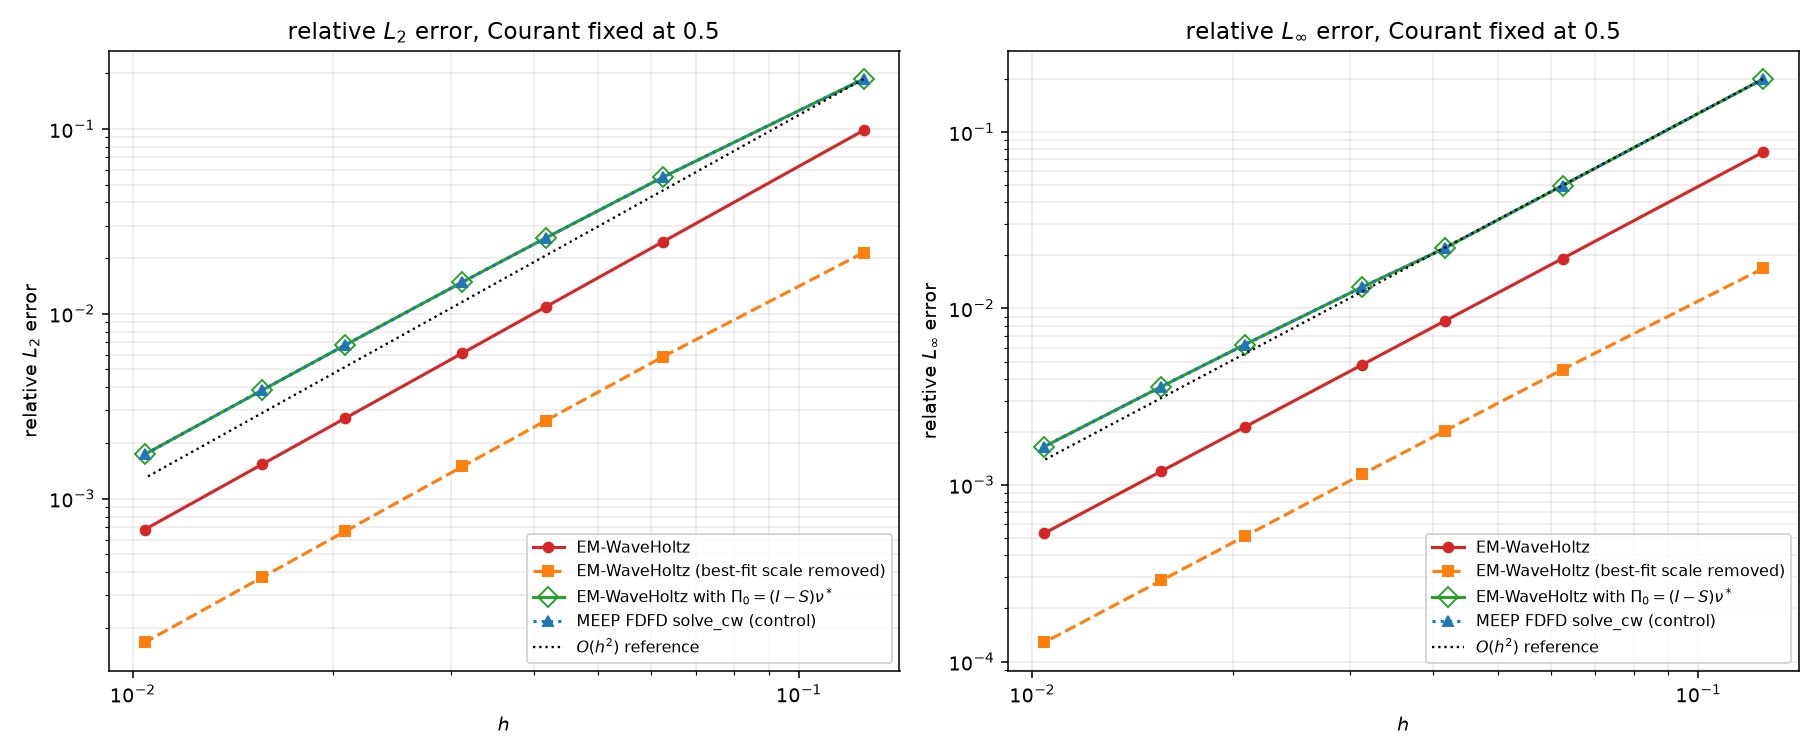
\includegraphics[width=\textwidth]{pec_convergence.png}
\caption{Relative $L_2$ (left) and $L_\infty$ (right) errors against $h$ at
fixed Courant number $0.5$. All series are second order; EM-WaveHoltz sits
below the FDFD control. Series~3 (open diamonds) lies exactly on the control,
as it must.}
\end{figure}

\clearpage
\section{Interpretation}
\label{sec:interp}

\paragraph{Initial data belongs in $D$ and $B$.}
MEEP time-steps the flux fields and recomputes $E = D/\varepsilon$ and
$H = B/\mu$ through \texttt{update\_eh} every step, so a write to $E$ or $H$ is
discarded on the next step. The consequence is not subtle: injecting a Gaussian
into $E_z$ in a lossless PEC box, where energy must be conserved, leaves
$\sum E_z^2 = 13.85 \to 0.039$ after a single step, while the same data injected
into $D_z$ gives $13.85 \to 12.82 \to 11.05$. With the write going to $E$, the
operator $S$ was close to the zero operator on the interior and the iteration
could not propagate initial data at all.

\paragraph{Why the earlier structural checks did not catch it.}
Worth recording, because each looked reassuring and none of them exercised the
operator. $I-S$ was symmetric positive definite --- but a near-zero operator is.
The spectral radius came out \emph{exactly} $0.5$, which is $|\beta(0)|$, the
multiplier of the \textbf{static} mode: the wave modes were being annihilated,
and that number should have been read as a symptom rather than a success.
Substituting $\Pi_0 = (I-S)\nu^\ast$ reproduced $\nu^\ast$ to $10^{-15}$ --- but
with $S \approx 0$ that identity reads $\nu^\ast \approx \nu^\ast$ and holds
regardless of whether $S$ is correct. Every one of these was invariant under
$S \to 0$. The check that settles it in one line is energy conservation of
freely evolving injected data.

After the fix the same tests describe a genuinely different operator:
$\rho(S) = 0.279$, a real wave mode rather than the static one; symmetry
$1.8\times10^{-16}$ on the \emph{full} grid rather than only the interior; and
the ghost ring completely decoupled, with zero leakage.

\paragraph{Series 3 is now a consistency check, not a diagnosis.}
Driving the iteration with $\Pi_0 = (I-S)\nu^\ast$ still reproduces
\texttt{solve\_cw} to round-off, as eq.~\eqref{eq:pi0} guarantees. With a correct
$S$ that is a meaningful confirmation that the operator, the filter and the
fixed-point driver agree with an independent solver; it is no longer evidence
about where any defect lives.

\paragraph{EM-WaveHoltz is more accurate than the FDFD control here.}
At res $96$ it reaches $6.8\times10^{-4}$ against $1.7\times10^{-3}$, roughly
$2.5\times$ better on the same grid, both at second order. The two solve slightly
different discrete problems --- MEEP's continuous-wave source is applied at
$t = \Delta t$ rather than at the half step $\Delta t/2$ that eq.~(23a)
specifies (measured amplitude $\mathrm{sinc}(\omega\Delta t/2)$ exactly, spatial
profile exact to $1.7\times10^{-16}$) --- so a difference at this level is
expected and is not evidence that either is wrong.

\paragraph{Remaining known gaps.}
The PML/ring configuration is disabled: with PML the current enters the
$D$-update and $E$ is reconstructed through auxiliary variables, so writing
$D$/$B$ is no longer equivalent to setting the state and the iteration diverges.
And the fixed point is $T$-periodic only to $4\times10^{-4}$, not to round-off,
most likely because the eq.~(24) half-step back-out has no stencil partner in the
last row and column, making the state round trip inexact at the grid edge.
Neither affects the convergence result above.

\section{Ring resonator with PML}

The closed-cavity study above fixes $\varepsilon=\mu=1$. The paper's Fig.~1
example does not: a ring resonator with $\varepsilon_r = 3.4^2$ on
$[-6,6]^2$, $1 \le r \le 2$, two antisymmetric $E_z$ point sources at
$(\pm1.1,0)$, $\omega_0 = 0.118\cdot2\pi$, closed here with MEEP's PML in place
of the paper's double absorbing layer. We use $\cos$-forcing and filter over
ten periods, as the paper does for this figure.

\paragraph{The state must be $(D,B)$, not $(E,H)$.}
MEEP time-steps the flux fields, so initial data is written to $D$ and $B$
(Sec.~\ref{sec:interp}). Where $\varepsilon \ne 1$ that distinction is no
longer cosmetic: filtering $E$ and injecting the result into $D$ drops a factor
of $\varepsilon$ throughout the ring. With an $(E_z,H_x,H_y)$ state the
iteration diverges at $61\times$ per application; with a $(D_z,B_x,B_y)$ state
it converges at rate $0.82$. Since $\varepsilon$ and $\mu$ are time
independent, filtering $D = \varepsilon E$ is exactly $\varepsilon$ times the
filter of $E$, so this is the same method written in flux variables; $E$ is
recovered at the end by injecting the converged state and reading $E_z$, where
MEEP applies $E = D/\varepsilon$.

\paragraph{Result.}
At resolution $10$ ($N=120$ across $[-6,6]$, matching the paper's coarsest
grid) the plain fixed-point iteration reaches a relative increment of
$10^{-8}$ in $93$ iterations and $41$~s; \texttt{solve\_cw} takes $3.6$~s.
No Krylov acceleration is used here, which is the bulk of that gap --- the
paper's Table~II counts are GMRES-accelerated.

\begin{figure}[h]
\centering
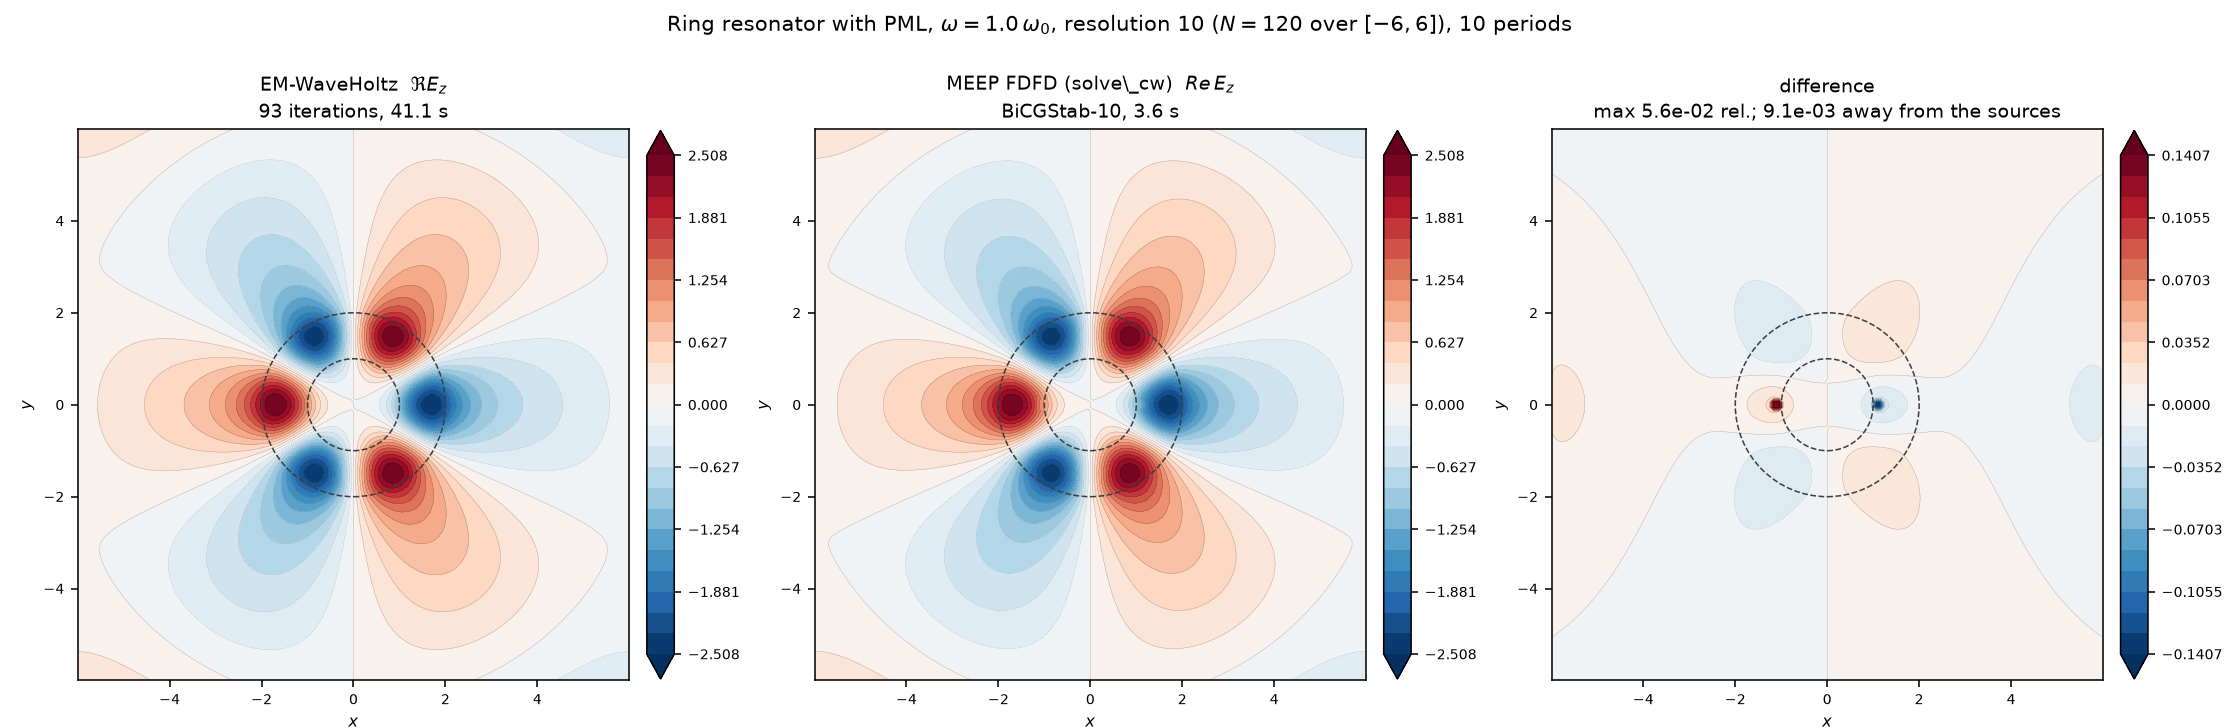
\includegraphics[width=\textwidth]{ring_compare.png}
\caption{Ring resonator, $\Re E_z$ at $\omega_0$. Left: EM-WaveHoltz. Centre:
MEEP's FDFD solver. Right: their difference, on the same colour scale
convention but its own range. Dashed circles mark the dielectric ring; only the
physical domain $[-6,6]^2$ is shown, the PML is cropped.}
\end{figure}

\paragraph{Where the two differ.}
The fields agree to $1\%$ over almost all of the domain. The max-norm
difference is $5.6\times10^{-2}$ relative, but it is concentrated in two spots,
exactly at the point sources: excluding disks of radius $0.6$ about
$(\pm 1.1, 0)$ it falls to $9.1\times10^{-3}$. That is expected --- a point
source is a delta function, neither solver converges pointwise at it, and the
two apply the current at slightly different instants (MEEP's continuous-wave
source acts at $t=\Delta t$ rather than the half step $\Delta t/2$ of
eq.~(23a)).

Two scans support that reading rather than blaming the PML. Increasing the
filter window at resolution $8$ leaves the max difference essentially
unchanged ($5.80, 5.50, 5.45 \times 10^{-2}$ for $5$, $10$, $20$ periods),
so it is not a PML-transient effect; and refining the grid does not reduce it
either ($5.7, 5.5, 6.4, 8.0 \times10^{-2}$ for resolutions $6, 8, 12, 16$),
which is what a non-convergent point singularity looks like in the max norm.
What \emph{does} converge with more periods is the overall amplitude: the
best-fit scale between the two solutions goes $1.0365 \to 1.0141 \to 1.0048$
for $5 \to 10 \to 20$ periods. That is the PML auxiliary variables, which sit
outside the filtered state and are reset every window; filtering longer lets
them settle, exactly the mitigation the paper relies on.

\section{Ring resonator: grid refinement in $L_2$}

The ring has no exact solution, so "error" needs a reference and the choice is
part of the result. Two independent measures are reported. First, the error
against a highly resolved \texttt{solve\_cw} (resolution $60$), which is cheap
and second-order convergent and so serves both methods. Second,
\emph{self-convergence}: successive differences between EM-WaveHoltz solutions
alone, which needs no reference and cannot inherit any bias from the FDFD
solver.

Everything is evaluated on a fixed point set --- the $E_z$ Yee lattice at
resolution $5$, restricted to $[-6,6]^2$. Resolutions $5, 10, 15, 20$ and the
reference $60$ are all multiples of $5$, so that lattice is a \emph{subset} of
every grid used and each solution is sampled exactly at those points: no
interpolation enters the comparison. $\|e\|_2 = (h^2\sum e^2)^{1/2}$, relative
to the reference. Because the two point sources are delta functions and neither
method converges pointwise at them, $L_2$ is also reported over the domain with
disks of radius $0.6$ about $(\pm1.1,0)$ removed.

\begin{table}[h]
\centering
\small
\begin{tabular}{rr rr rr rr}
\toprule
& & \multicolumn{3}{c}{EM-WaveHoltz} & \multicolumn{3}{c}{MEEP FDFD}\\
\cmidrule(lr){3-5}\cmidrule(lr){6-8}
res & $h$ & iters & rel $L_2$ & rate & time & rel $L_2$ & rate\\
\midrule
 5 & 0.2000 & 82 & 1.644e-1 & ---   &   9.1\,s & 1.758e-1 & ---  \\
10 & 0.1000 & 81 & 5.451e-2 & 1.593 &  42.5\,s & 4.927e-2 & 1.835\\
15 & 0.0667 & 83 & 2.481e-2 & 1.942 & 135.6\,s & 1.970e-2 & 2.261\\
20 & 0.0500 & 83 & 1.537e-2 & 1.664 & 288.3\,s & 1.005e-2 & 2.339\\
\bottomrule
\end{tabular}
\caption{Ring resonator at $\omega_0$, ten periods, measured against
\texttt{solve\_cw} at resolution $60$. Excluding the source disks changes every
entry by less than $4\%$ and is omitted. The EM-WaveHoltz iteration count is
flat in resolution.}
\end{table}

\begin{figure}[h]
\centering
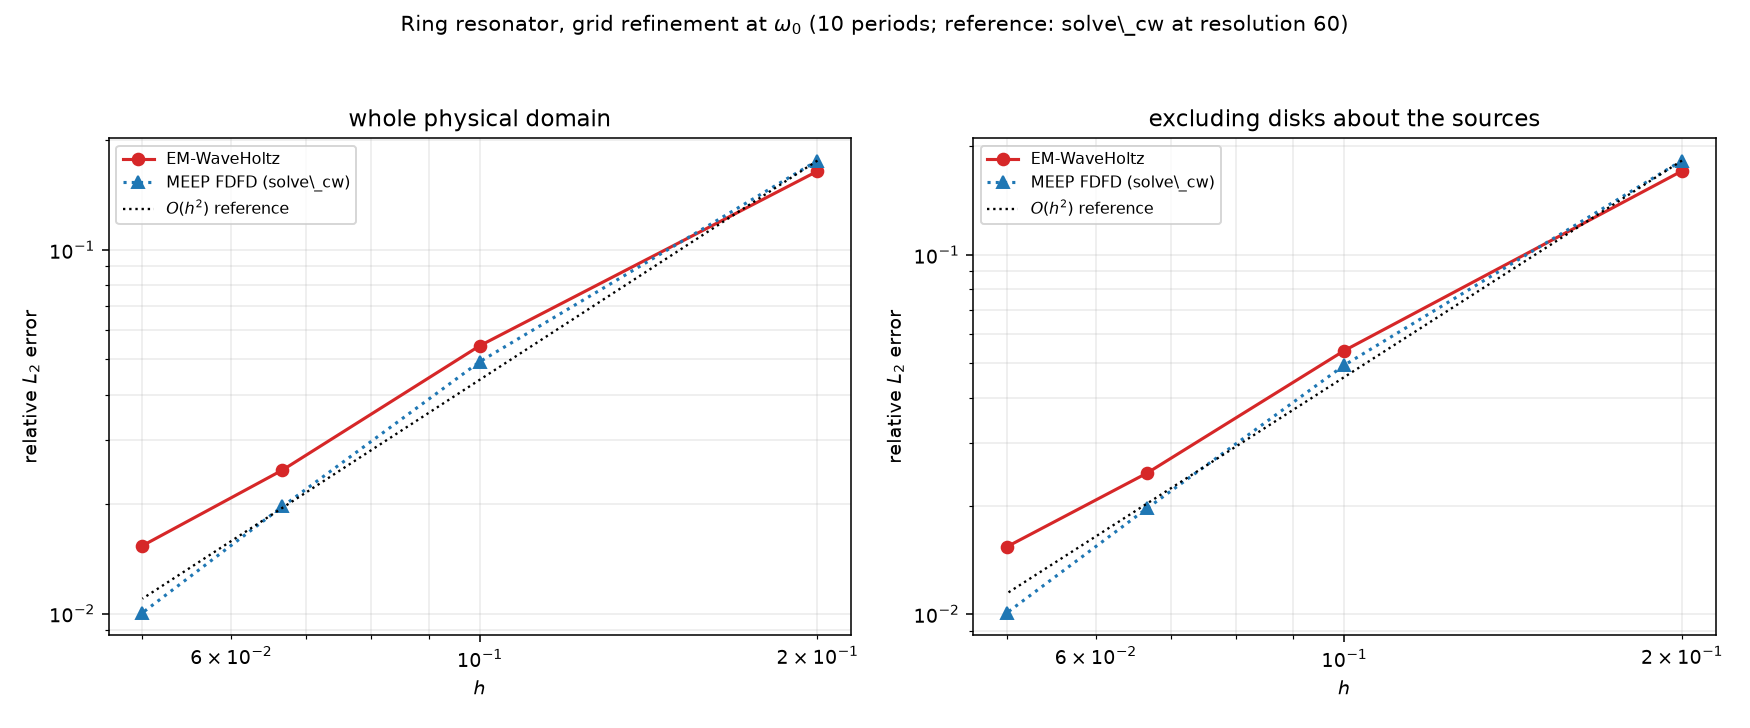
\includegraphics[width=\textwidth]{ring_refine.png}
\caption{Relative $L_2$ error against $h$ for the ring, over the whole physical
domain (left) and excluding disks about the two point sources (right). Both
methods track $O(h^2)$.}
\end{figure}

\paragraph{The reference-based rates are contaminated; read them with care.}
The FDFD column reports rates of $2.26$ and $2.34$, above two, which cannot be
an asymptotic order. It is an artefact of measuring a method against itself:
with $e_{\text{ref}} \approx (r/60)^2 e_r$ and the same error shape, the
measured difference is $e_r(1 - (r/60)^2)$, which is suppressed more at fine $r$
and inflates the apparent rate. The same mechanism has the opposite sign for
EM-WaveHoltz, whose error does not cancel against the reference's, depressing
its last rate to $1.66$. The finest points are therefore the \emph{least}
trustworthy in this table, not the most.

\paragraph{Self-convergence, which has no such defect.}
\begin{center}
\small
\begin{tabular}{lrr}
\toprule
& whole domain & excluding sources\\
\midrule
$\|u_5 - u_{10}\|_2 / \|u_{\text{ref}}\|_2$    & 1.5855e-1 & 1.6503e-1\\
$\|u_{10} - u_{15}\|_2 / \|u_{\text{ref}}\|_2$ & 3.2057e-2 & 3.2004e-2\\
$\|u_{15} - u_{20}\|_2 / \|u_{\text{ref}}\|_2$ & 1.0685e-2 & 1.0631e-2\\
\bottomrule
\end{tabular}
\end{center}

\noindent For a $p$-th order method the successive difference is dominated by
the coarser grid,
\begin{equation}
  \|u_a - u_b\|_2 \;\sim\; C\,a^{-p}\big(1 - (a/b)^p\big),
  \label{eq:selfconv}
\end{equation}
and the refinement ratio here is not constant ($2$, $1.5$, $1.\overline{3}$).
Fitting eq.~\eqref{eq:selfconv} gives $p = 1.853$ from the first pair of
differences, $p = 2.136$ from the second, and $p = 1.880$ from a least-squares
fit over all three: \textbf{second order}, in agreement with the closed-cavity
study. (Taking a plain $\log$ ratio of successive differences instead, which
drops the $1-(a/b)^p$ factor, reports a spurious $3.8$ on this same data. That
is worth stating because it is the natural thing to compute and it is wrong
whenever the refinement ratio varies.)

\paragraph{Cost.}
The EM-WaveHoltz iteration count is essentially independent of resolution ---
$82, 81, 83, 83$ --- which is the behaviour claimed in the paper's Table~II.
Wall-clock time still favours BiCGStab at these sizes, because the iteration
here is a plain fixed point with no Krylov acceleration. The FDFD advantage
does not persist: \texttt{solve\_cw} takes $0.6, 5.7, 17.1, 39.6$~s at
resolutions $5$ to $20$, but $1740$~s at resolution $60$ --- a factor of $44$
for $9\times$ the cells, so its iteration count is growing by roughly $5\times$
over that range while EM-WaveHoltz's does not grow at all.

\section{Reproduction}

\begin{verbatim}
conda activate meep
python scripts/convergence_pec.py   # notes/pec_convergence.png
                                    # notes/pec_convergence_data.txt
python scripts/probe_pi0.py         # direct Pi0 comparison at one resolution
python scripts/ring_compare.py      # notes/ring_compare.png
python scripts/ring_refine.py --resolutions 5 10 15 20 --reference 60
                                    # notes/ring_refine.png (~38 min)
\end{verbatim}

Relevant code: \texttt{emwh/manufactured.py} (exact solution, forcing, norms),
\texttt{emwh/core.py} (the iteration), \texttt{scripts/convergence\_pec.py}
(this study), \texttt{scripts/probe\_pi0.py} (the $\Pi_0$ diff).

\end{document}
